%%% Fiktivní kapitola s ukázkami sazby

\chapter{Návrh řešení}

V této kapitole je popsáno technické řešní uvedených problémů.

\section{Odhad zpoždění}

\subsection{Současná řešení}

Algoritmus na odhat aktuálního zpoždění mezi dvěma referenčními body již exituje a je součástí Datové Platformy -- Golemio, ze kterého se čerpají data pro tuto práci. (Detailní popis dat uveden v kapitole ~\ref{chapter:TODO later}.)

\bigbreak

Nicméně tento algoritmus nijak nezohledňuje variabilitu profilu trasy. Totiž v tomto řešení je nahlíženo na postup vozidla na trase jako na lineární funkci vůči času. Je ovšem zřejmé, že rychlost vozidel není konstantní, neboli doba jízdy není linárně závislá na ujeté vzdálenosti.

\bigbreak

Proto je potřeba tento odhad zpřesnit, což je cílem naší práce. K tomuto cíli jsme byli nasměrování v rámci schůzky s pracvoníky společnosti OICT, kde bylo řečeno, že toto je problém současného řešení, který je potřeba vyřešit. 

\subsection{Funkční požadavky}

\begin{itemize}
	\item
Popsaný odhad změny zpoždění na trase mezi dvěma referenčními body je nutné počítat v co nejkratším čase tak, aby cestující byli dobře informování o stavu jejich spoje a mohli tyto informace využít např. při dobíhání spoje. A proto je potřeba zpracovávat data okamžitě po jejich vydání, spočítat odhad zpoždění a vystavit tato data veřejně. Vzhledem k tomu, že tato data velmi rychle zastarávají je nutné provádět tento proces co možná nejrychleji\footnote{Průměrná doba jízdy spoje mezi zastávkami je cca 5 min. Rozložení počtu úseků mezi zastávekami k délce jízdy mezi nimi je závislé a podobné rozložení vůči vzdálenosti ilustrované na grafu\ref{fig:stop_distances_result}.}.

\item

Data o polohách vozidel VHD v Datové platfomě jsou aktualizována nejpozději každých 20 sekund, více v kapitole \ref{chapter:analyza_zdroje}. Tedy pro minimalizaci rychlosti zastarávání dat a získání všech existujících vzorků dat o polohách je nutné data stahovat alesponˇ každých 20 sekund.

\item

Odhad zpoždění se bude provádět na základě historických dat z posledních vyšších jednotek dnů\footnote{Pro demonstrativní účely této práce jsou využívány historická data pouze ze 4 dnů (2 pracovní a 2 víkendové).}. Tím se sníží dopad mimořádné události na předpovědní model, která může na trase vzniknout. Zárovenˇ by však neměla být započítávána data starší několik týdnů, protože dopravní situace se mění v závislosti na ročním období nebo také pokud je na trase delší omezení dopravy je požadováno, aby se takové omezení projevilo co možná nejdříve. Navíc se bude rozlišovat mezi daty z pracovních dnů a nepracovních dnů, to protože samotné jízdní řády se mohou lišit (doba jízdy mezi mezastávkama) a také se do velké míry liší hustota dopravy, která ma velký vliv na profil jízdy. TODO do navrhy na zlepseni: Pro zpřesnění výsledků by bylo lepsi respektovat svatky, kazdy den v tydnu zvlast atp.

\item

Zpracování historických dat bude probíhat vždy po delší době, nejlépe jednou za den. To umožní provádět náročnější výpočty, které by za normálního provozu neúměrně přetížily systém. Navíc vzhledem k povaze cíle práce ani není žádoucí zpracování historických dat provádět častěji než jednou denně, protože se nepokoušíme okamžitě reagovat na změnu dopravní situace.

\item

Uložená historická data budou struktorovaná tak, aby nad nimi šly provádět statistické výpočty minimálně o frekvencích spojů, vzdálenostech tras, zpoždění spojů.
\end{itemize}

\subsection{Kvalitativní požadavky}

\begin{itemize}

	\item
	Řešení bude schopno při jedné aktualizaci zpracovat alesponˇ 1000\footnote{20. 2. 2020 mezi 7:00 a 7:10 bylo na trase přes 600 vozidel} vzorků poloh vozidel, kde 10 \% vzorků může být o dosut neznámých jízdách. V tomto případě je potřeba stáhnout jízdní řád konkrátní jízdy a její jízdní profil, což navíc dotaz na zdroj dat.

	\item
	Vypočítané modely profilů jízd budou dávat odhat zpoždění lepší, než je lineární odhad. To znamená, že zpoždění vypočítaná pro každý přijatý vzorek polohy vozidla mezi dvěma referenčními body na trase bude mít menší rozptyl než lineární odhad zpoždění.

\end{itemize}




\section{Vizualizace dat}

\subsection{Funkční požadavky}

Součástí práce je i vizualizace spočítaných dat.

\bigbreak

To bude provedeno formou front endové aplikace, která zobrazuje mapu a do ní zanáší data o vozidlech VHD. Funkční požadavky této aplikace jsou inspirované již existujícími řešeními tohoto problému.

\subsection{Současná řešení} \label{chapter:soucasna_reseni_front_end}

Vizualizaci vozidel \gls{vhd} do mapy již nabízí několik portálů. Všechny jsou však poměrně strohé.

\subsubsection{Golemio}

Takovou mapu zobrazuje i samotný provozavatel datové platformy. Nicméně nejsou zde vidět ani čísla linek zobrazených autobusů, natož pak nějaké další informace.

\begin{figure}
  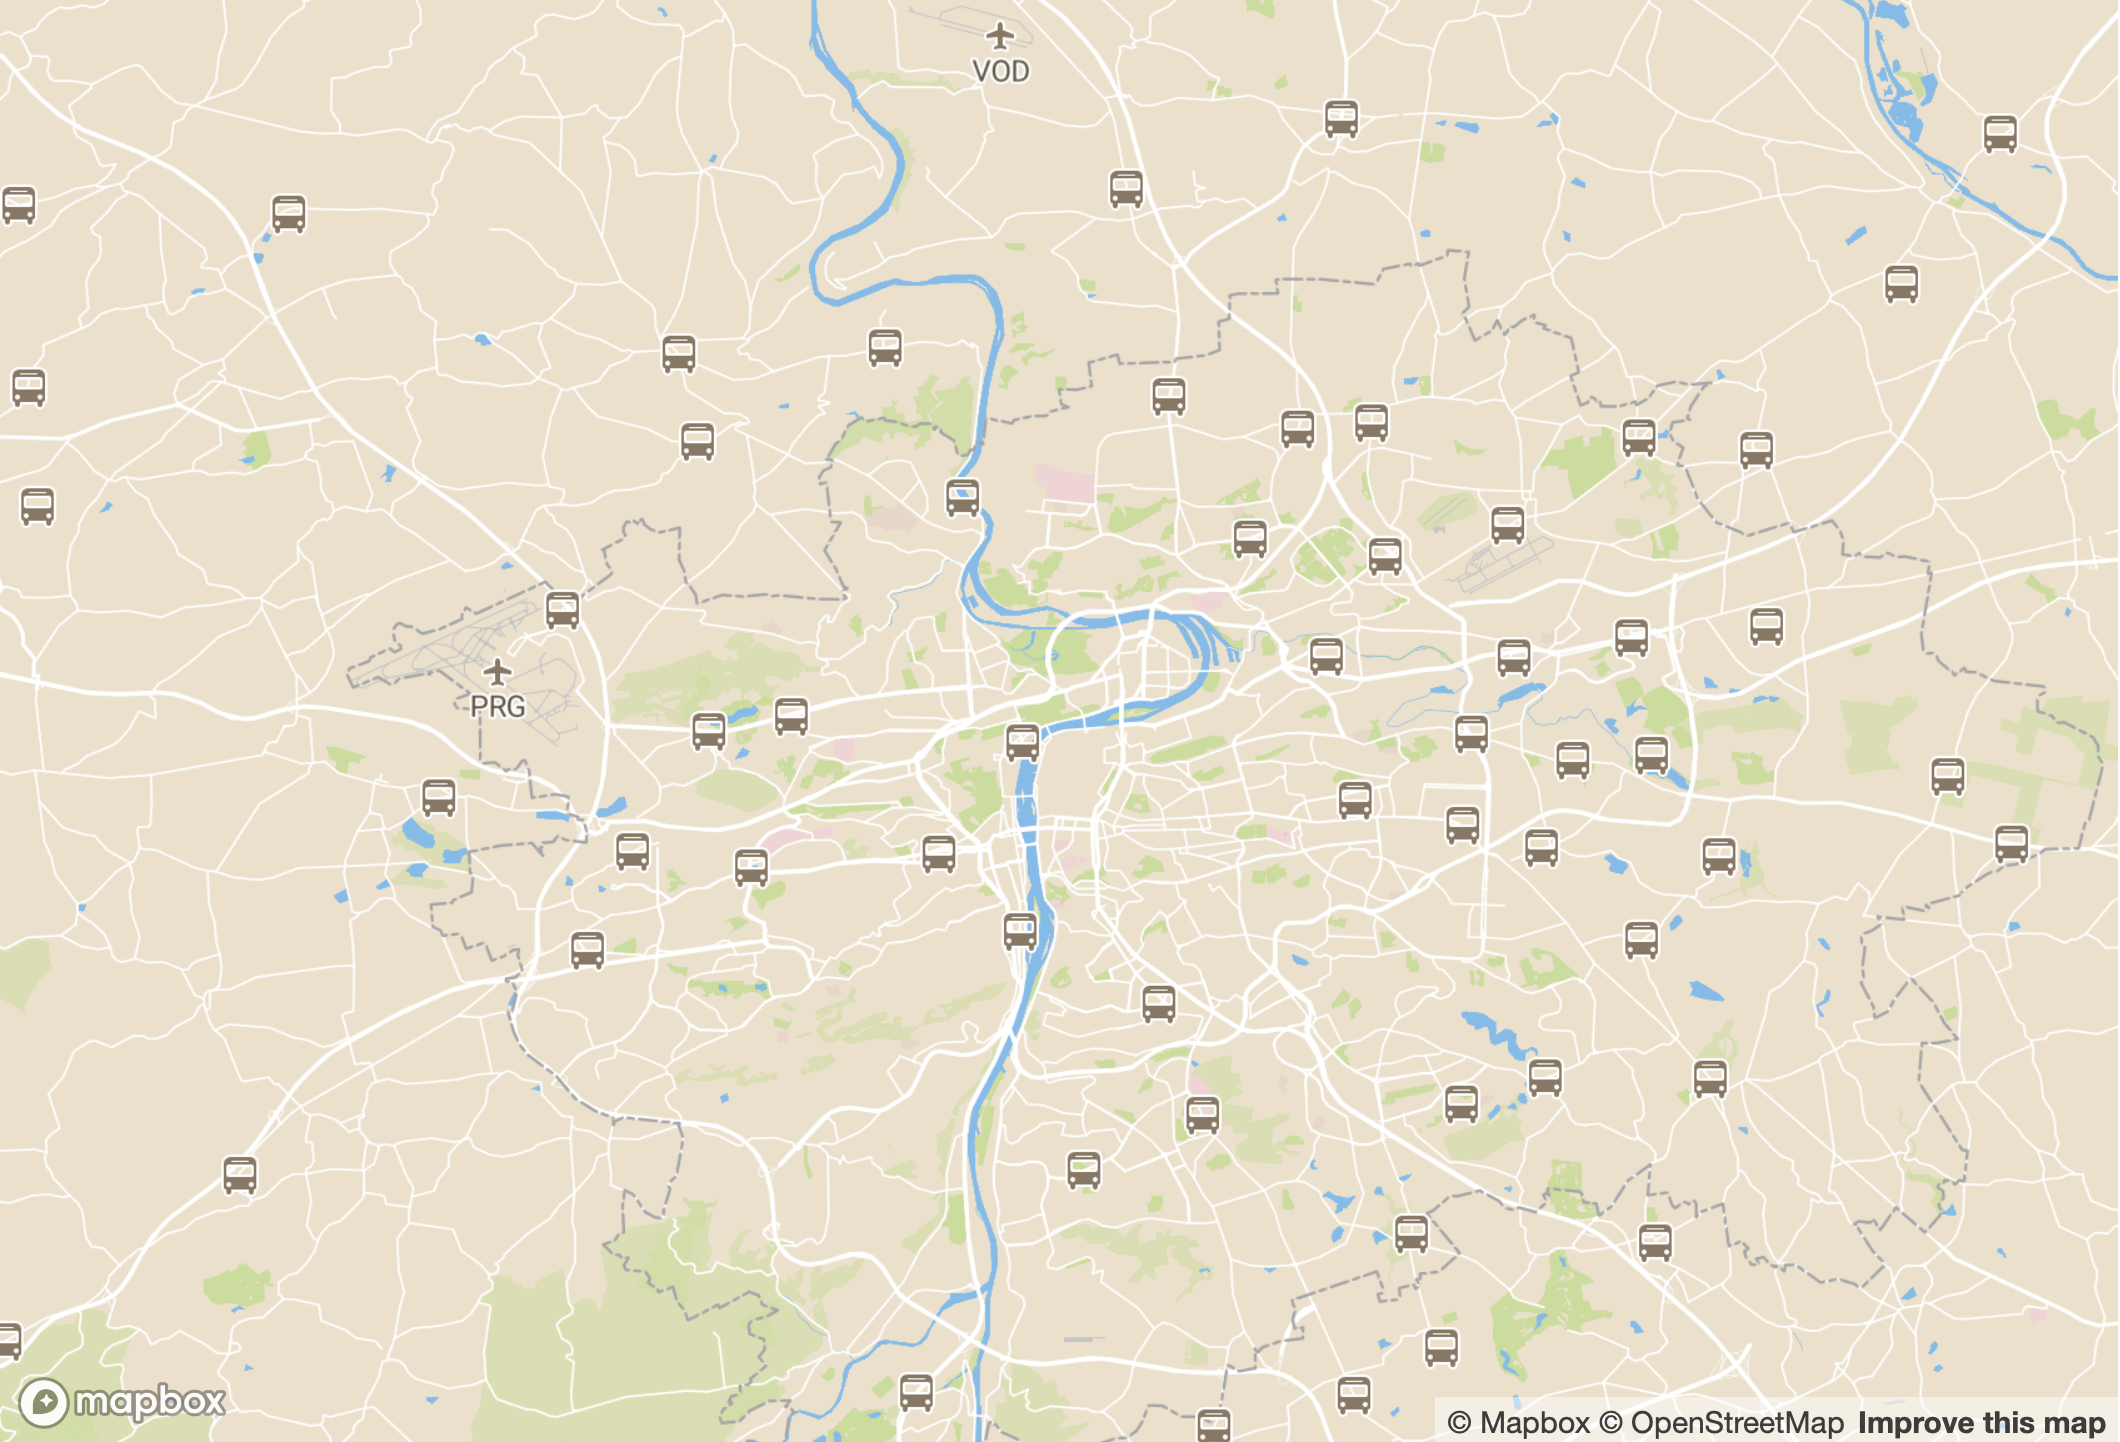
\includegraphics[width=\linewidth]{../img/golemio_mapa.png}
  \caption{Mapa z golemio.cz.}
  \label{fig:golemio_result}
\end{figure}

\subsubsection{Tram-bus}

Dalším poskytovatelem je portál tram-bus, který si vede o něco lépe. Ukazuje směr jízdy vozidel, čísla linek a po kliknutí informace o zpoždění a nejbližší zastávky. Pozn.: na mapě již jsou vidět spoje \gls{dpp}, protože v době psaní této práce již byly data veřejné.

\begin{figure}
  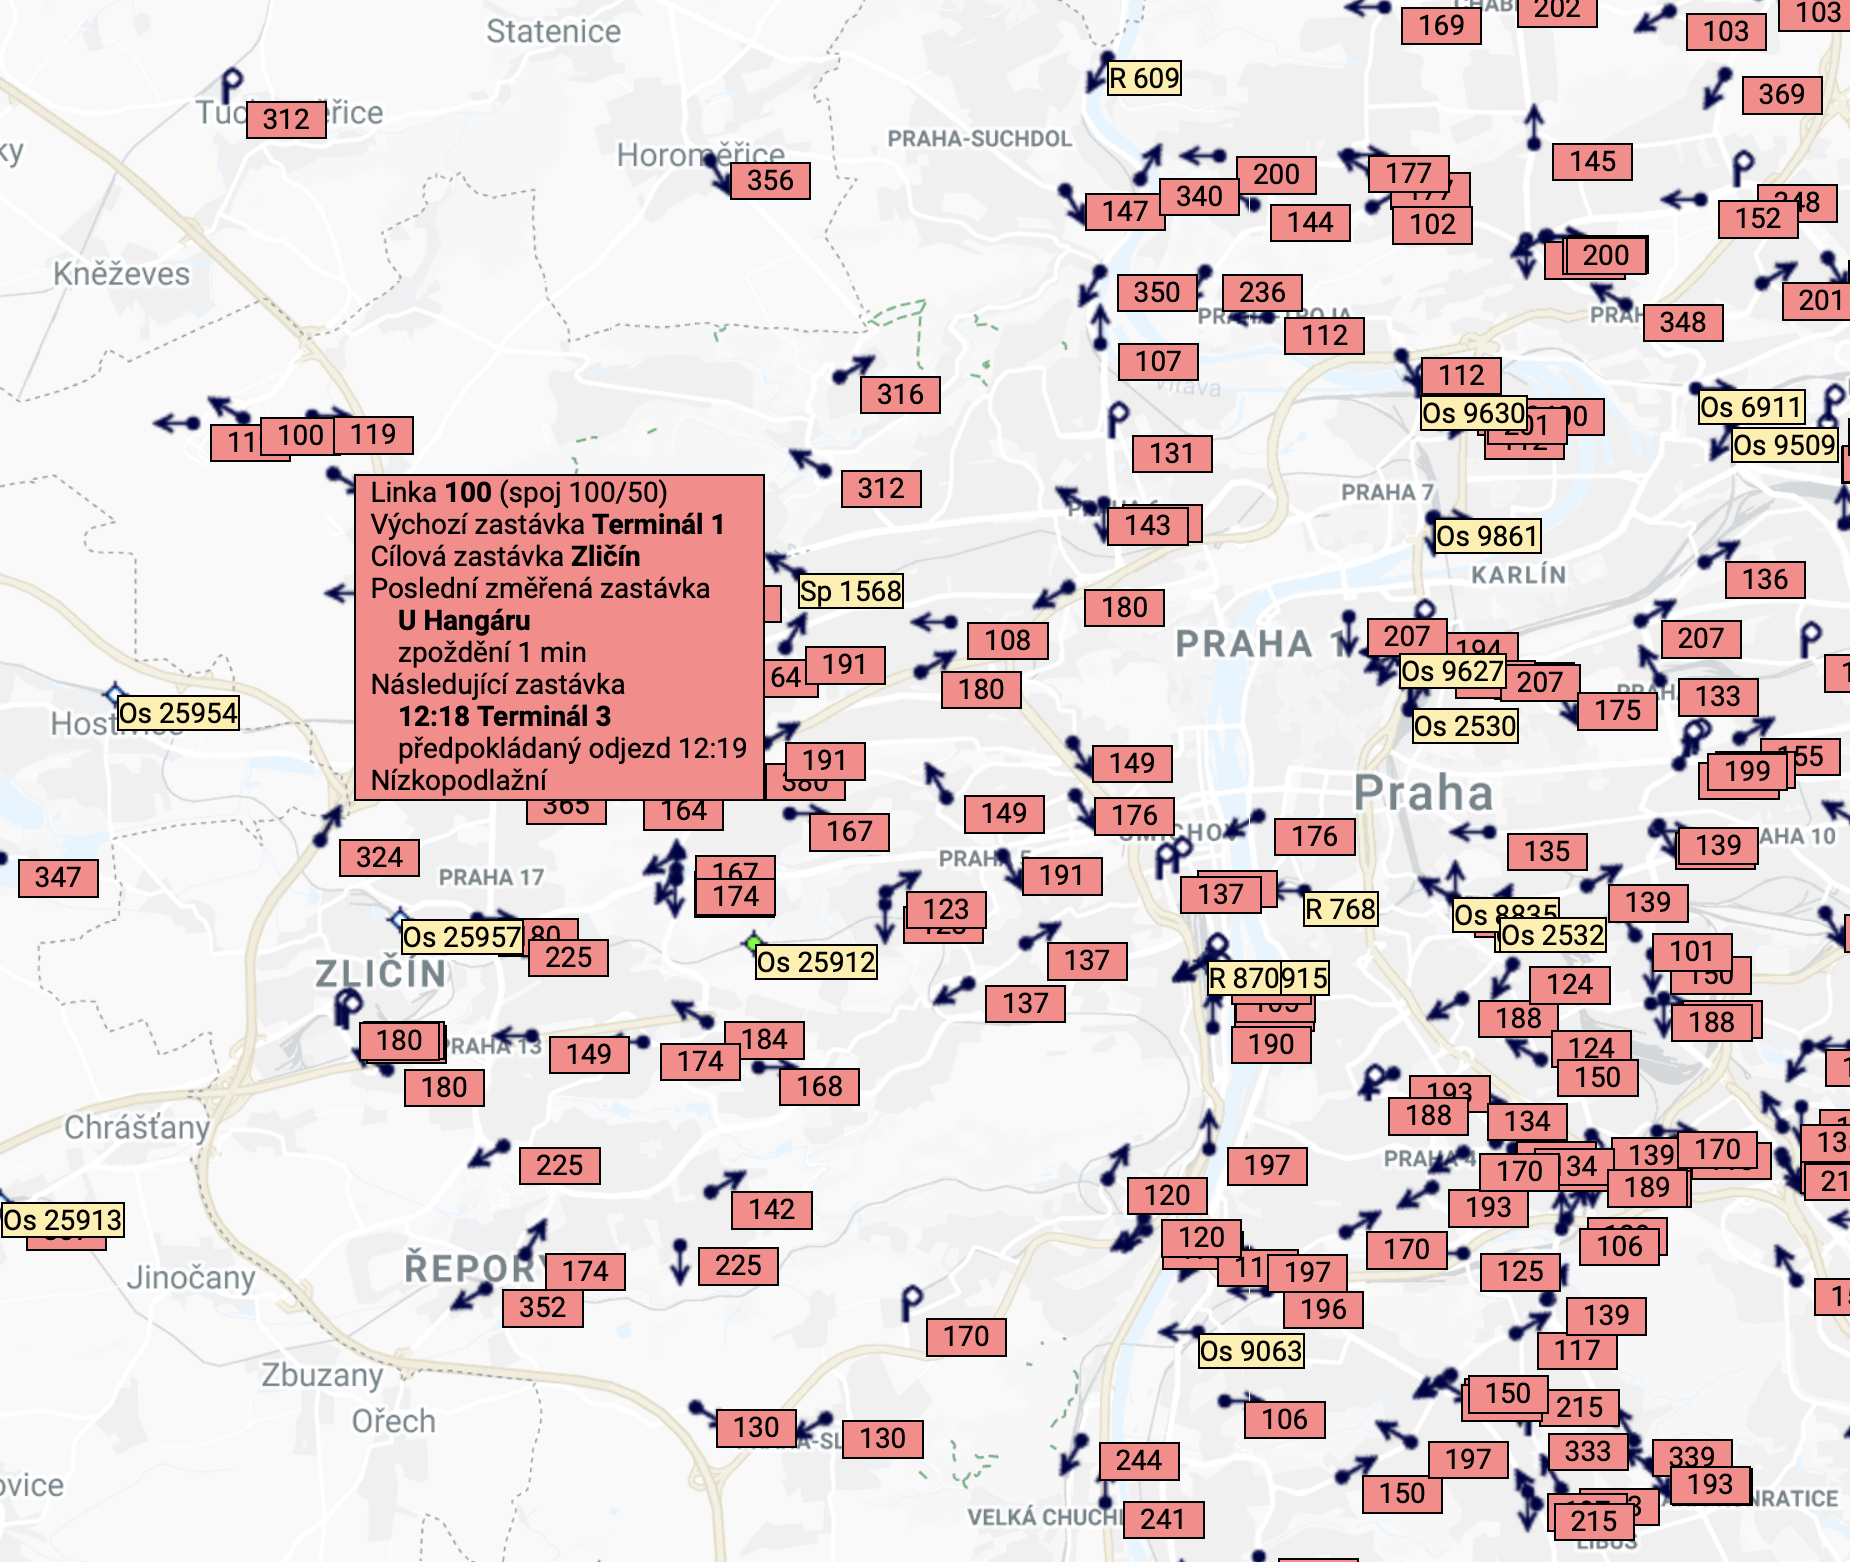
\includegraphics[width=\linewidth]{../img/tram-bus_mapa.png}
  \caption{Mapa z www.tram-bus.cz.}
  \label{fig:tram-bus_result}
\end{figure}

\subsubsection{\gls{idsjmk}}

Mimo Prahu je velice pěkně udělaná aplikace pro zobrazení vozidel \gls{idsjmk} (Integrovaný dopravní systém Jihomoravského kraje). Ten ihned po načtení stránky zobrazuje všechny dobravní prostředky, tedy tramvaje, autobusy a vlaky vše s čísly linek. Dále pak umožňuje po kliknutí na vybraný spoj zobrazit více informací včetně jízdního řádu.

\bigbreak

Tato aplikace je po vizuální i funkční stránce dobrou inspirací pro tvorbu aplikace v této práci.

\begin{figure}
  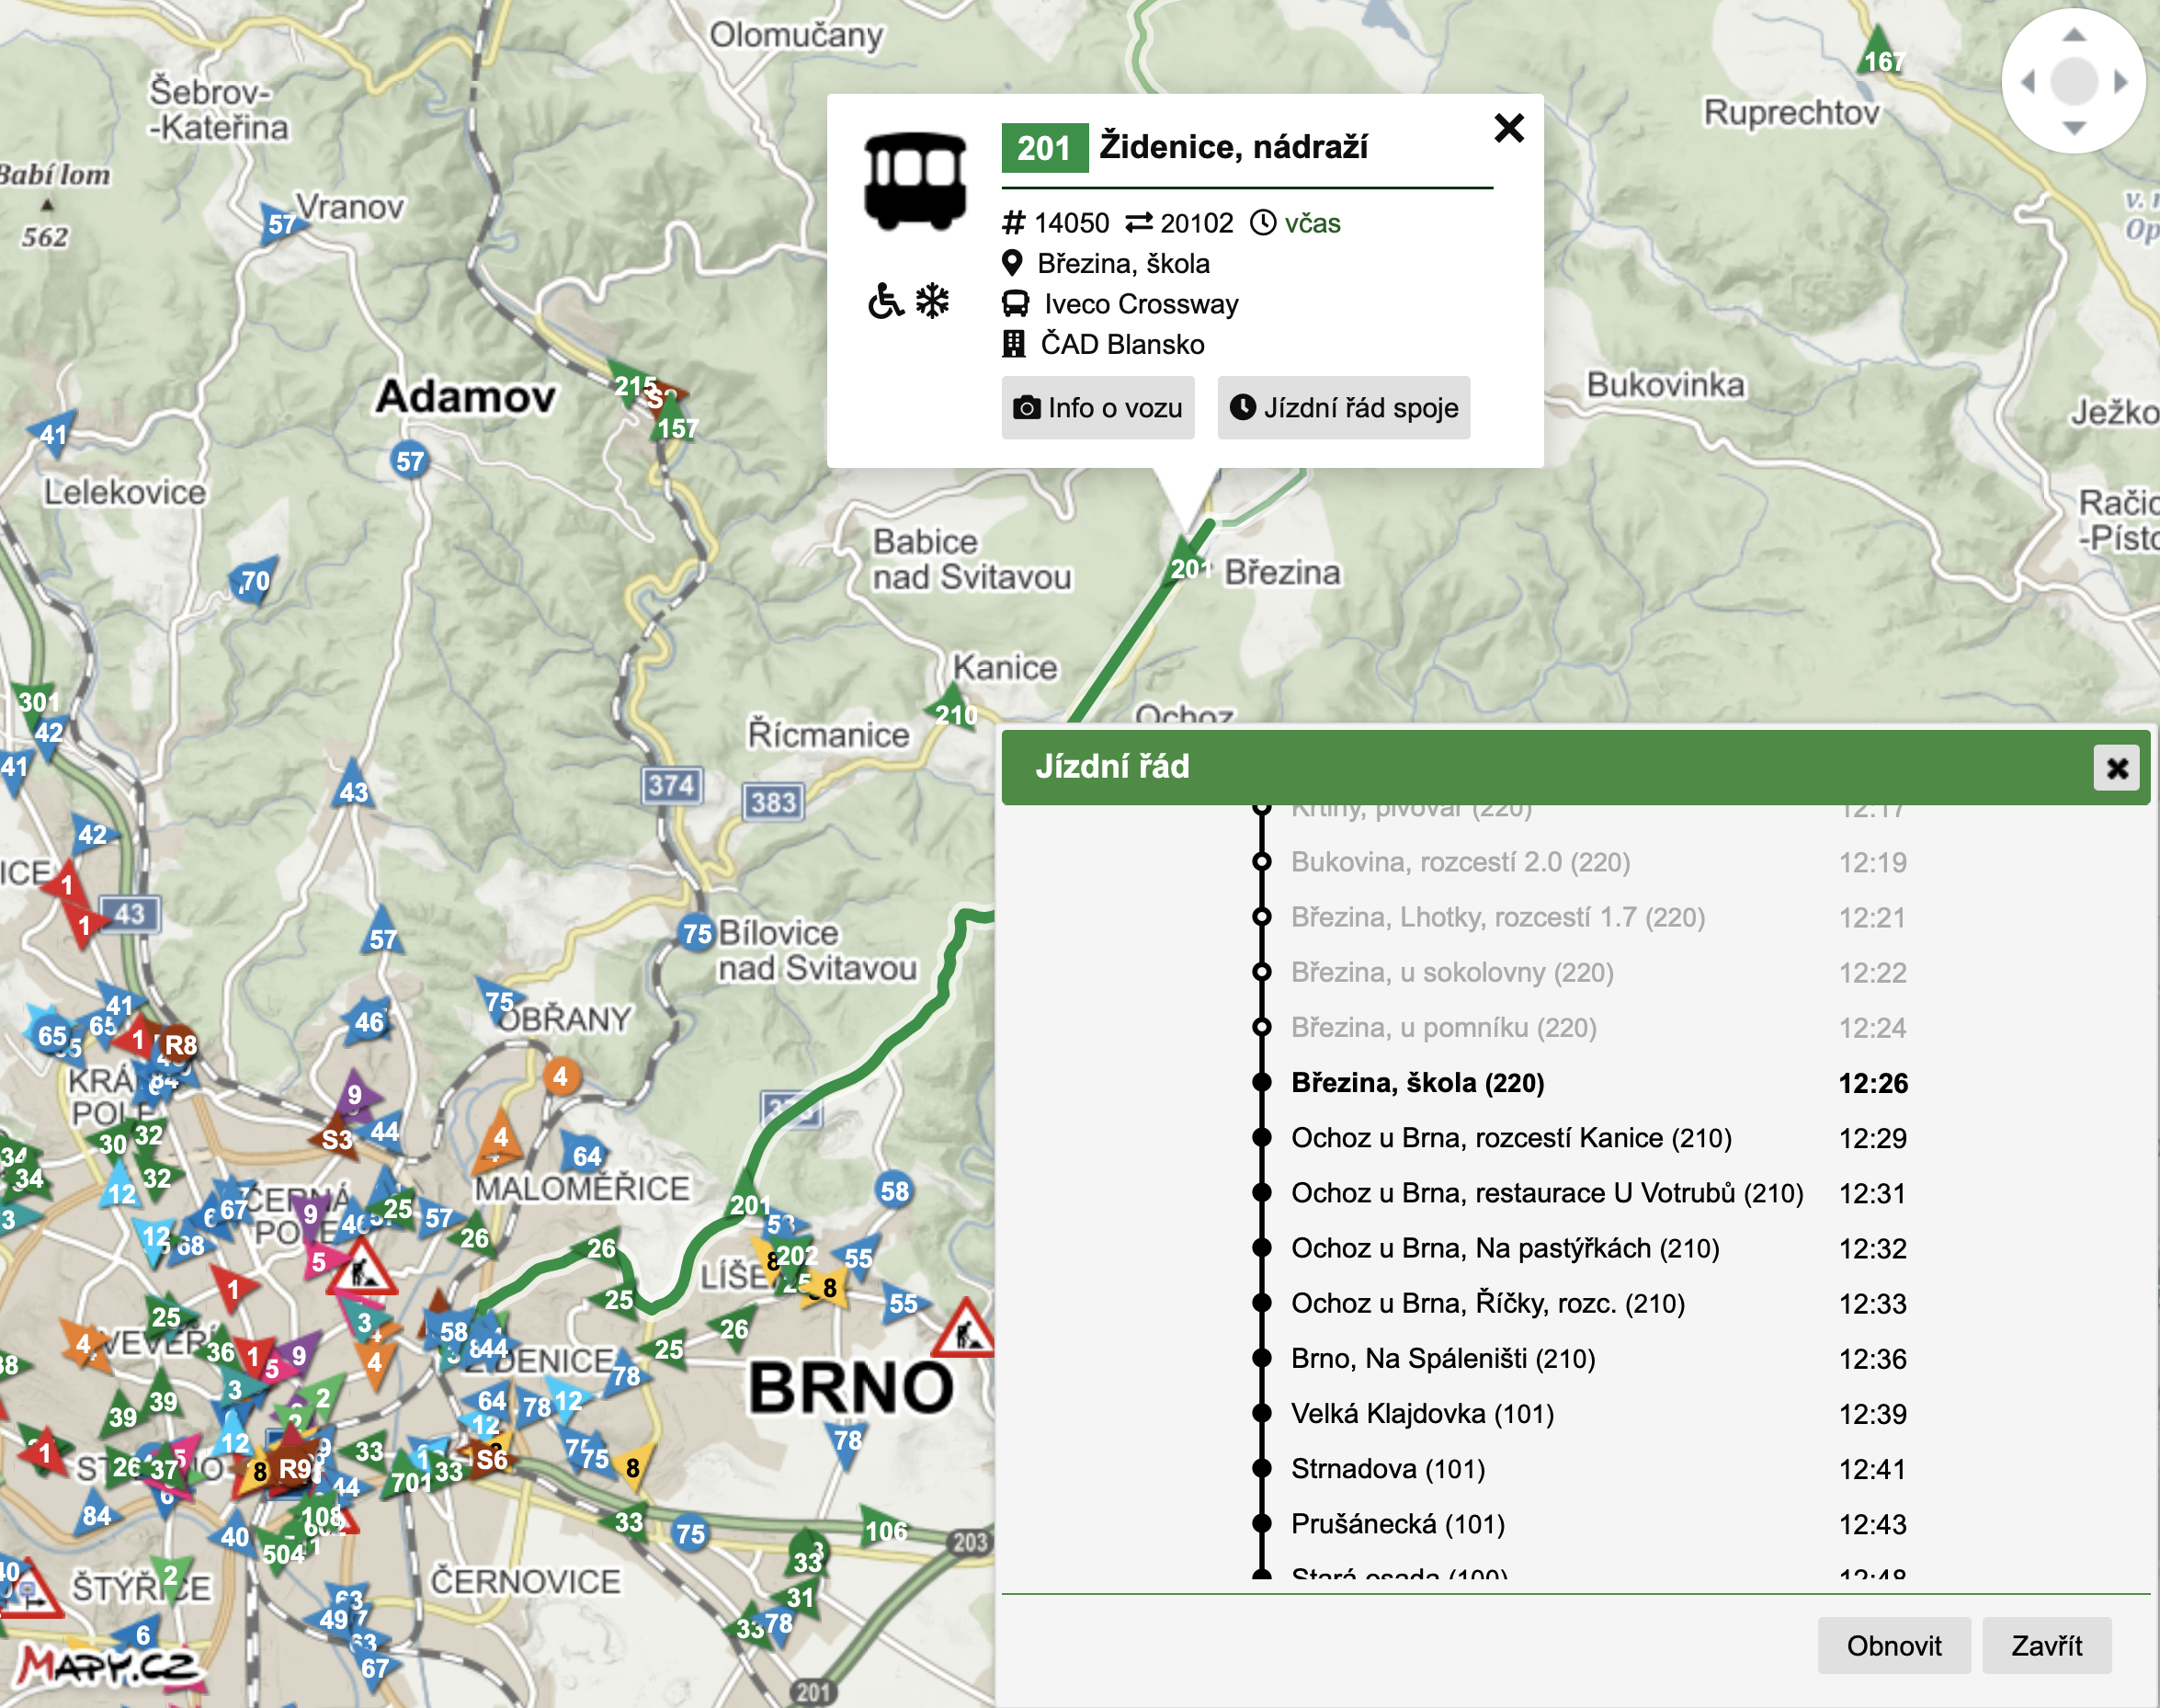
\includegraphics[width=\linewidth]{../img/idsjmk_mapa.png}
  \caption{Mapa z mapa.idsjmk.cz.}
  \label{fig:idsjmk_result}
\end{figure}

\subsection{Funkční požadavky}

\begin{itemize}
	\item

	\item Aplikace vykreslí interaktivní mapu Prahy a širšího okolí, kterou bude možné posouvat či zoomovat. V této mapě budou zobrazeny vozidla na aktuálních pozicích a budou se automaticky posouvat po mapě, tak jak se pohybují ve skutečnosti.

	\item Po kliknutí na vozidlo se zobrazí jeho celá trasa včetně zastávek a jeho dopočítaného zpoždění.

	\item Po kliknutí na zastávku se zobrazí seznam spojů, které budou projíždět vybranou zastávkou a jejich trasy se vykreslí do mapy.

	\item Celá aplikace bude postavena na principu server -- client. Tedy serverová strana se postará o přístup k otevřeným datům o vozidlech a jejich uložení a také obsluhu požadavků klienta. Klientská část bude webová stránka poskytující služby popsané výše. Měla by být schopná zobrazit řádově tisíce vozidel.
\end{itemize}

\subsubsection{Nefunkční požadavky}

\begin{itemize}
	\item Serverová část bude napsaná v jazyce Python 3.

	\item Webová část bude napsaná pomocí jazyků pro webové technologie, převážně v JavaScriptu.

	\item Pro vykleslení mapy bude využita služba Mapbox.

	\item Ukládání dat na serverové straně bude řešeno MySQL databází.

	\item Pro algoritmus odhadu zpoždění na zákldě historických dat budou využity různé knihovny pro jazyk Python 3. Zejména pak scikit-learn a alphashape.

\end{itemize}

\subsubsection{Proces běhu aplikace}

Jak je již zmíněno aplikace bude využívat historická data, tedy bude nutné nechat aplikaci tato data nějakou dobu sbírat. Pro efektivní odhady by bylo vhodné mít uložené historické polohy vozidel alespoň z uplynulých několika týdnů.

\bigbreak

Avšak již v průběhu sběru dat může aplikace poskytovat základní službu a to vizualizování vozidel v mapě.

\subsection{Poskytovatelé mapových podkladů}

K takovému účelu nejlépe poslouží vykreslení aktuálních poloh vozidel do mapy, kde se po vyžádání uživatelem tyto data zobrazí.

\bigbreak

Za účelem vytvoření dostatečně přívětivé uživatelské aplikace je nezbytné využít některého z poskytovatelů mapových podkladů a zanést do něj získané informace.

\bigbreak

Jedním z těchto poskytovatelů je společnost Google, která má propracované mapové podklady a prostřednictvím služby Google Maps poskytuje pro tuto práci požadovanou službu. Další platformou je Mapbox, který poskytuje velmi podobné služby jako Google Maps. Nicméně narozdíl od Googlu využívá jako mapový podklad \gls{osm} {otevřená geografické data}. Protože smyslem práce je v co největší míře využít otevřená data je žádoucí využít právě Mapbox.

\bigbreak

TODO dokumentace mapbox, zeptat se jestli je to vubec nutne rozebirat
